\documentclass[12pt, a4paper]{memoir} % for a short document
\usepackage[english]{babel}
\usepackage [vscale=0.76,includehead]{geometry}              
\usepackage{fullpage}
\usepackage{mathptmx} % font = times
\usepackage{helvet} % font sf = helvetica
\usepackage[latin1]{inputenc}
\usepackage{relsize}
\oddsidemargin 0.0cm  
\evensidemargin 0.0cm  
\textwidth 17cm 
\topmargin -1cm 
\textheight 23.5cm
\usepackage{graphicx}
\usepackage{float} 
\usepackage{multimedia}
\usepackage{amsmath,amssymb}
\usepackage{listings}
\usepackage{graphicx} % Allows including images
\usepackage{booktabs} % Allows the use of \toprule, \midrule and \bottomrule in tables
%\usepackage[nottoc, notlof, notlot]{tocbibind}
\usepackage{amsfonts}
\usepackage{amsmath,bm}
\usepackage{hyperref}
\usepackage[round]{natbib}
\lstset{
  numbers=left,   
  firstnumber=1,
  numberfirstline=true,
  language=C, 
  frame=L
  } 



\bibliographystyle{plain}

%\headstyles{komalike}
\nouppercaseheads
\chapterstyle{dash}
\makeevenhead{headings}{\sffamily\thepage}{}{\sffamily\leftmark} 
\makeoddhead{headings}{\sffamily\rightmark}{}{\sffamily\thepage}
\makeoddfoot{plain}{}{}{} % Pages chapitre. 
\makeheadrule{headings}{\textwidth}{\normalrulethickness}
%\renewcommand{\leftmark}{\thechapter ---}
\renewcommand{\chaptername}{\relax}
\renewcommand{\chaptitlefont}{ \sffamily\bfseries \LARGE}
\renewcommand{\chapnumfont}{ \sffamily\bfseries \LARGE}
\setsecnumdepth{subsection}


% Title page formatting -- do not change!
\pretitle{\HUGE\sffamily \bfseries\begin{center}} 
\posttitle{\end{center}}
\preauthor{\LARGE  \sffamily \bfseries\begin{center}}
\postauthor{\par\end{center}}

\newcommand{\jury}[1]{% 
\gdef\juryB{#1}} 
\newcommand{\juryB}{} 
\newcommand{\session}[1]{% 
\gdef\sessionB{#1}} 
\newcommand{\sessionB}{} 
\newcommand{\option}[1]{% 
\gdef\optionB{#1}} 
\newcommand{\optionB}{} 

\renewcommand{\maketitlehookd}{% 
\vfill{}  \large\par\noindent  
\begin{center}\juryB \bigskip\sessionB\end{center}
\vspace{-1.5cm}}
\renewcommand{\maketitlehooka}{% 
\vspace{-1.5cm}\noindent
\includegraphics[height=14ex]{logoINP.png}\hfill\raisebox{2ex}{
\includegraphics[height=7ex]{logoUJF.jpg}}\\
\bigskip
\begin{center} \large
Master of Science in Informatics at Grenoble \\
Master Math\'ematiques Informatique - sp\'ecialit\'e Informatique \\ 
option \optionB  \end{center}\vfill}
% End of title page formatting

\option{$<$GVR$>$}
\title{ Inverse Procedural Generation of Geological Stories}%\\\vspace{-1ex}\rule{10ex}{0.5pt} \\sub-title} 
\author{Garcia Maxime}
\date{ $<$June 23rd 2016$>$} % Delete this line to display the current date
\jury{
Research project performed at $<$INRIA Monbonnot$>$ \\\medskip
Under the supervision of:\\
$<$Dr. R\'emi Ronfard ,INRIA$>$\\\medskip
Defended before a jury composed of:\\
$[$Mr$]$ $<$George-Pierre Bonneau$>$\\
$[$Mr$]$ $<$James Crowley$>$\\
$[$Mr$]$ $<$Edmon Boyer$>$\\
$[$Mr$]$ $<$Jean-Sébastien Franco $>$\\
$[$Mr$]$ $<$last-name$>$\\
}
\session{$[$June$]$\hfill 2016}

\begin{document}
\selectlanguage{english} % french si rapport en français
\frontmatter
\begin{titlingpage}
\maketitle
\end{titlingpage}

\section{Abstract}

This thesis addresses the problem of restoring the complete history of a 2D geological 
subsurface also called a cross-section. It is a key problem for geologists when they want to understand how the terrain transformed to be in state it is today. Moreover it allows them to date geological events such as faults, erosion or sedimentation. It is also a major issue for oil searchers because by looking at the cross section evolution they can deduce places where oil is likely to be trapped in. Tools to tackle this problem have already been created and can  be caterogized into two kinds: geometrical based tools which deform the initial cross-section relying only on geometrical and kinematical property of the drawing and physical based ones which focus on runninng a simulation using physical equation applied to the section in order to deform it. However those tools usually restore only one scenario of the cross-section history when several of them can exist.\\\\
 Here, we propose a new hybrid method which focuses on proposing multiple scenarios of the cross section restoration. As an input we will take a cross section drawing containing topological data and we will map mass spring system on it, which will be the center of our animation process. In addition we will propose the user to choose among possible events to transform the cross section to its restoration state and simulate the selected ones. Each time an event simulation end we ask the user to make another event choice until there are no event to propose left. One main feature of our methods is that the user is able to come back to its previous choices and create an other scenario as he pleases in order to build a tree of scenarios which we will call a story tree.\\\\
 
\section{Introduction}

Hand-drawn sketches are very used in geology for illustrating and validating hypotheses. It is the main way of keeping and showing geological data. Indeed, showing an image of what we have in mind is a really good way to convey our thoughts, especially here in geology where we can draw from multiple points of view. Futhermore geologists write lots anotations on their drawing to give more hints and be more specific in the information they want to show in their sketchs. 
For instance sketches can be used to reconstruct a 3D view of the subsurface by drawing a 2D top view of the current terrain (2) and using anotations or to represent 2D vertical cross-sections. \\\\

However anotations are limited in explaining what happened in the past, it is difficult to anotate the past of the geological representation on a single sketches. Therefore geologists must draw several sketches when they whant to show the history of a terrain. \\\\

This exaclty what they do when they want to do cross section restoration (ref). It consists in drawing several sketches of the same cross section at different time steps starting from the its current state. A cross section is composed of several geological elements, in particular blocks, layers and faults. The layers they draw correspond to different sedimentary layers that have deposited  along history. Blocks correspond to parts of the section which are between two faults or one fault and on boundary of the sketch. Finally faults correspond to breaks in the section and create discontinuities in it. They can be of three types:
Normal, Reverse or Strike-slip. Normal and Reverse faults correspond to vertically oriented breaks which make blocks slide among their left or right side. Normal faults happen during extension while reverse one happen during compression. As for Strike-slip faults, their are horizontal breaks that make blocks sliding on their bottom or upper parts.\\
However as we are in the 2D vertical case we are only interesed in the reverse and normal faults.\\\\
Here is an exemple of a geological sketch: 
%Chartreuse
\begin{figure}[H]
	\centering
	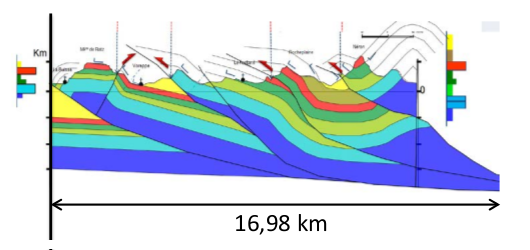
\includegraphics[scale=0.8]{Wraped_Section.png}
	\caption{Chartreuse Cross Section}
\end{figure}

The current state of the cross section is the result of several geological phenomena such as erosion, foldings, sedimentations, fault impacts, etc..., which occured in the past at different time. Consequently, restoring a cross section can differ depending on the geologist point of view.\\\\
However using the initial sketch  and geometrical tools (ref) geologists are able to draw the past state of the cross section before any erosion, fault and sediment events and this restoration is usually unique and doesn't differ much between geologist.An analysis of the different layers and faults usually lead to the same geometrical evolution reconstruction which has been provoqued by compression or extension of the rock masses before, after or during deposit and erosion of the sediments and basement rocks. \\\\

The main problem geologist are facing in this restoration is to find (deduce) what really happened to go from the current state to the past one. They have two things to identify. First they have to find all the events that occured from the past to the current state. Then they have to find in with order they occured because it is possible that even when changing the event order we obtain the same restoration at the end. Futhermore it is possible to find the same restoration having identifying different events in two different hypothesis. \\\\

Consequently geologists have to draw lots of sketches in order to expose their hypothesis. In addtition those drawings are rather limited: on top of representing only one 2D cross-section of the terrain being investigated, they can only represent hypotheses on the underground geometry at discrete time steps, rather than a complete continuous history. Futhermore insuring consistency between these sketches over time heavily depends on available data, maturity of the regional geological interpretation and the skills of the geologist, i.e. his knowledge on the way rocks and sediments fold, on the way faults propagates and produce sliding and displacements, and on the way sediments are deposited or eroded, etc...\\\\


Recently, it was proposed to organize geological sketches into story trees to present and compare different interpretations of the formation of a given terrain (6) but the task remains labor-intensive, requiring the geologist to draw every sketch in the story tree. Moreover, even while being skillful and experienced, it’s hardly impossible to a geologist to express a continuum of the deformation of a geological cross-section with available tools.
In this internship, we would like to follow up on this line of research by proposing methods for inferring a geological story tree directly from one geological sketch, and presenting the resulting tree of possible geological stories as an animation.\\\\

\section{State of the Art}\\

Several solutions of very different kind have been proposed to solve the problem of correctly exposing many restoration hypothesis without inconsistencies and without spending too much time creating them. We distinguish two types of solutions: the geometrical ones and the mecanical ones.\\\\

Geometrical solutions consist in assuring only geometrical consistancy when exposing the solution while mecanical ones consist in running a physical simulation over the past cross section and see if the animation created confirm the hypothesis.\\\\

\section{Geometrical solutions}

Like mentionned above Lidal (ref) proposed a solution using trees to organize their resoning. Starting from the initial drawing the geologist can draw several stories where each node of the tree conctains a new sketch. In addition it is possible to superimpose the previous drawing to the new one helping keeping geometrical consitancy and reducing conciderably the time spent for drawing. Futhermore as geologists use usually seismic recording to draw the starting drawing, having this recording in background really help them in being consitent.\\\\
 As a result with fewer sketches and less time spent in drawing, geologists (see eg) can express their ideas better than with traditionnal sketching. Futhermore this tool is really efficient when exploring different hypothesis  because at each node we can create another branch to explore a new possibility and thus they can either refined their animation or try different scenarios. \\\\

However this solution doesn't necessarely keep the topological consistancy of drawing unless the geologist spend more time being carefull of having precise topological consistant drawings. This topological aspect can be important when validating hypothesis especially when they restore very old cross sections and the topology of the terrain underwent drastic changes(exemples?).\\\\\

Recently VAC and VGC proposed a solution to have space-time topological consistancy in 2D drawings. More precisely it propose a solution for inbetweening two drawings of the same model which underwent topological changes. The fondation of the technique is the data structure VGC which has been shown to model all possible incidence relations between vertices, edges and faces in 2D sketches. Then the VAC are used to describe all possible changes in the topology of a vector graphic complex over time(exemples?).\\\\\

Other geometrical tools such as "move 2D" (ref) are used  to produce the restoration. They use geometrical and geological properties of the drawing and apply kinematic algorithms to deform the different blocks and units. They take into account several geological phenomena such as compaction, erosion, sedimentation and folding in order the keep the geological consistancy while the user is restoring interactively the cross section. They also consider more specific effects such as thermal subsidence and isostasy to have finer results in the restoration. As a result they produce sequences like:

\begin{figure}[H]
	\centering
	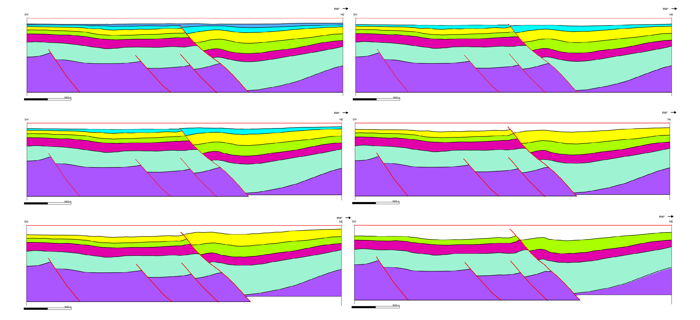
\includegraphics[scale=3]{mve2D.png}
	\caption{MVE 2D restoration sequence}
\end{figure}

 In addition this kind of tool can be used for foward modeling which can help geologists to validate their hypothesis in the case they want to check if the restoration they produced can give the same result as today terrain situation. Futhermore they can consider the 3D aspect of a subsurface using several cross sections and a 3D model of the considered area.\\\\\
  It is important to note that this kind of tool doesn't produce realisitc results in terms of physical aspect but they have fast computation time and let the user interact to build the restoration.\\\\\

Here is an example of the chartreuse restoration using this kind of geometrical tools:

%Chartreuse
\begin{figure}[H]
	\centering
	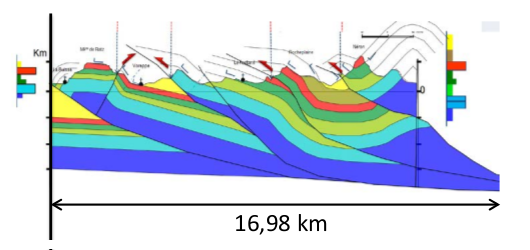
\includegraphics[scale=0.8]{Wraped_Section.png}
	\caption{Chartreuse Cross Section}
\end{figure}

%Chartreuse unWraped
\begin{figure}[H]
	\centering
	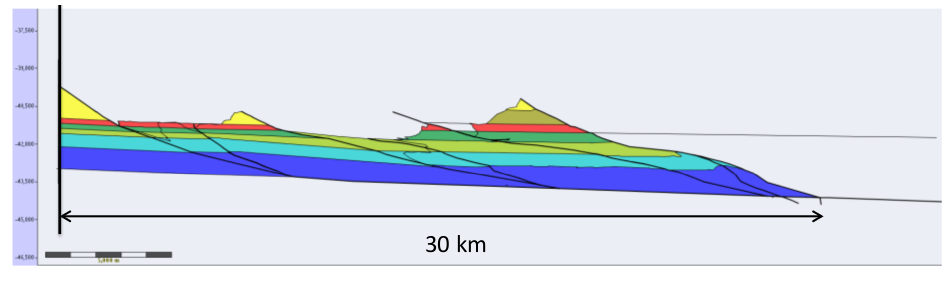
\includegraphics[scale=0.6]{UnWraped_Section.png}
	\caption{Chartreuse Restoration}
\end{figure}

 Here it was done manually by a geologist who  dealt with each block one by one and flattened each layer while conserving their respective height and area. After the flattening operation the user can manually stick the new block to its neighbours with the corresponding moduli facing each other.

\section{Physical solutions}

In order to solve the cross-section restoration problem an other kind of solution tools has been explored which is physically based tools. While geometrical tools don't assure the physical consistancy of the restoration which can question the restoration inbetweening , physical based tools are by nature physically consistent.\\\\

 We can identify two kind of physically based tools: those which help validating complex structural model of 3D subsurface like LithoTect (ref) and those which run a simulation over simpler but physically coherent enough using finite element method with the Coulomb theory like SLAMTec and OptumG2.\\\\
 
Software like LithoTect are very usefull because they allow geologist to build very consistent and complex model of a subsurface which implies that they can create very fine 2D cross section where they can run a physical simulation on it.\\\\

Software like SLAMTec or OptumG2 run simulations over simpler models which are also physically consistent but the simulation will take less parameters and properties of the terrain, leading to faster computation time.\\
Such tools can be used to validate a restoration. Indeed by running a simulation over the restoration geologist can see if what they produce seems coherent with the current state of the cross section even if those simulations can never produce the same result as this current state.\\\\
 This is one drawback of using those tool of forward simulation, even if we have a very fine representation of our model it can never achieve to retrieve a very similar correspondances and cannot validate by itself a restoration, geologists have to discuss the solution proposed.\\\\ 
 However some physically based tool try to  solve this problem by proposing a backward simulation. This simulation is not simulating the "real" inverse of what happened to the current cross section but they run a finite element simulation with opposite forces and condition to what the geologist think that happened. For instance if the current section has been subject to compression forces the tool will apply extension forces to the model, same thing with compaction and other phenomena.\\\\
 Here is an example of "Dynel 2D" (ref) which implements this method:
 \begin{figure}[H]
	\centering
	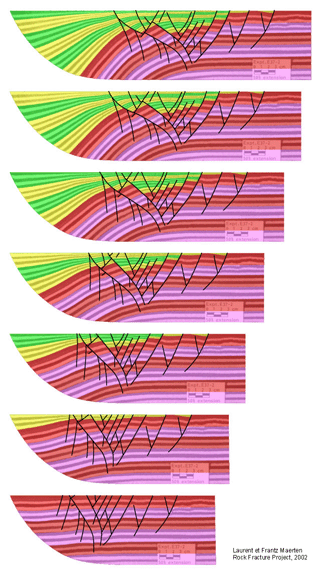
\includegraphics[scale=0.5]{dynel2D.png}
	\caption{Dynel 2D restoration sequence}
\end{figure}

 
 While this method is likelly to produce much better results in terms of similarity with the restoration and the current state of the section, it is more difficult to use because there exist many uncertainties on identifying the events that occured between the current cross section and the restoration as there are several possible scenarios. \\\\\

Even though those physically based tool respect physic laws and produce very consistent results, they are not fully matching the cross section current state and thus cannot validate the hypothetical section history they have simulated. In addition this kind of tool doesn't explore several scenarios and are restrained to a single or very few cases. 
That's why one of the main purpose of this master thesis is to explore and propose several plausible scenarios.

\section{Our Solution}

We presented two kinds of tools used for solving the problem of producing the animation between the recovered restoration and the current cross section. Moreover we can note that regardless the type of tool some of them produce forward animation and others backward ones. \\\\\
Here we will opt for a backward simulation using a hybrid tool between geometrical physical.Thus we will run an inverse modeling animation on the current 2D section and compare it visually to the provided restoration.\\\\

In this master thesis the main objective is to create a generic and interactive tool which builds different scenarios from a given drawing. The tool must give the user choices to make and allow him to come back on them. That's why similarly to Lidal (ref) we will use story trees to encode our scenarios.\\\\

More generally the tool we want to create is bind by the structure of the input data, the enconding of our story and scenarios, the way of animating the drawing and the validation method. Because we also want our tool to be interactive, we need to propose an animation model which is fast enough to make its computations in a near real time way. Basically, the general workflow we will follow is: \\\\1) Import the input drawing\\\\ 2) Choose a scenario to play \\\\3) Simulate it \\\\ 4) Evaluate its plausibility 5) Loop on the scenario step while the user wants to explore different stories\\\\

In our geological case we encounter lots of different topological configuration in the cross-sections. Indeed as we mentionned before our cross-section is composed of sedimentary layers, fault and blocks which are chunks of the section located between faults. Consequently each block contains part of superimposed layer which are called geological units (units for short) and their side show discontinuities with its neighbouring block. Each layer is colored with a unique color representing the period it has deposited. Topologicaly speaking our cross-section is a convex graph composed of faces representing the units, which means that every face as at least one neighbour and there are no isolated group of faces. The discontinuities we find in the cross section are due to faults creation caused by extreme folding conditions.\\\\

%drawing
 \begin{figure}[H]
	\centering
	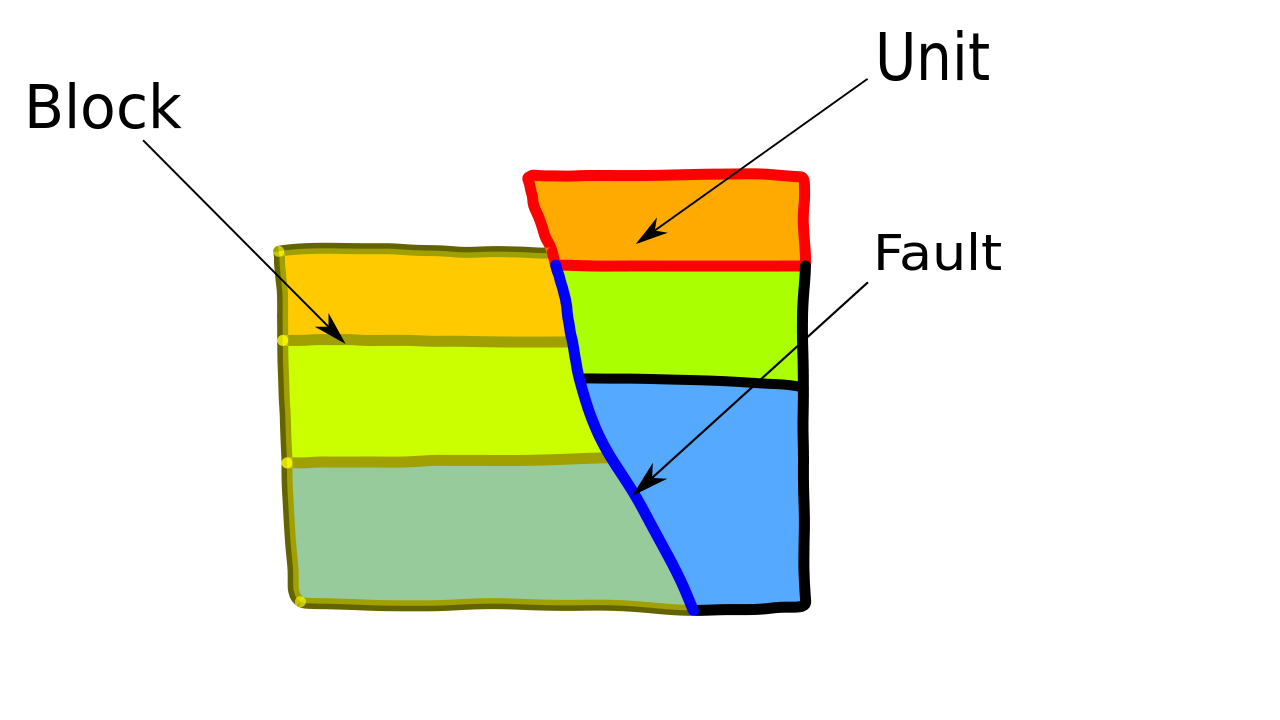
\includegraphics[scale=0.3]{geologyStructEdit.png}
	\caption{Cross section structure}
\end{figure}


Because of the cross section has a well defined topological representation and because it is changing over time we opted for using VAC and VGC structures which we allow us to keep a time-space topological consistency during the animation. The VGC data structure has the advantage of modeling all possible incidence relations between vertices, edges and faces in 2D sketches, therefore it is a good choice for us who want to produce a tool which can be applied to other situations outside the geological field. The VAC structure is used to animate the VGC and describe all possible changes in the topology of a VGC over time which is be a good solution to show our produced animation. As the VAC works with keyframing and inbetweening the keyframes we need to propose an inbetweening methods for our input model which will be part of our animation method.\\\\
  Because we use VGC and VAC structures all the input cross section will be drawn using the vpaint software (ref) which build a XML file as output. Then we will parse this XML file as the input of our tool.\\\\
%introduce vocabulary and global methods with schemes


Regarding the story telling part we propose a method similar to Lidal (ref) using a story tree. Each node of the tree corresponds to a cross section state in the time (going backward) where we can choose to simulate several events amoung a list of possible event at this particular time and state when each branch corresponds to the animation of the simulated events.
In our geological case we have to consider a set of events that impacted on the cross section we consider. In this master thesis we will consider the following ones: erosion, sedimentation, folding and faults. Thus because we are going backward in time we will try to undo thoses events and we will propose to the user either to un-erode, un-sediment, un-fold or un-fault the cross-section at a story tree node. \\\\


When the user choose undo events we have to simulate its effect. In order to do so we will use a first approximation of terrain displacement. We will consider sedimentary layers to be plastic materials. Thus as a first approximation we will map mass spring systems to our drawing in order to animate it. We will use a implicit euler scheme as the main animation loop and apply external transformation if needed for un-doing an geological event.\\\\

The validation can be done visually by the user but we also give him hints about the success rate. Indeed one important assumption that geologist often do is that the sedimention always occur with the upper bound of the new layer being horizontal. Because the last event to undo will be sedimentation we can give the user a deformation rate of the spring which will tell him to what extend the layer is horizontal (see continuous simulation). We can give this indication to the user each time we wants to do an un-sedimentation.\\\\

Futhermore it is possible that by choosing one path in the tree, the user meets a dead end without getting to the restoration state. This means that chosen sequence was not plausible at some point and the user must go back to its choices.\\\\

To summerize our general workflow is: first analysing the input vpaint drawing in order to extract all the geological structure we need to run our simulation on and propose plausible scenarios. Because we will need prior geological information for the simulation and to propose plausible events to the user, we ask the user to give some geological features of the cross section such as the layers' age, their deformation coefficient (Young Modulus ref), their friction coefficient and so on.\\ 
After this step, we map mass spring system on the cross section and propose the first events to undo at the root of the story tree. 
Then the user will choose progressively which events he wants to simulate and will build the tree of scenarios i.e. the story tree. At each step the user can go back to a previous node and decide to simulate other events that the ones he selected.
Finally during the simulation we will save the animation as VAC in an output XML file in order to have a fluid animation.\\\\

\section{Cross section data structure and Drawing analysis}

As mentionned above our input drawing will be built using vpaint software which implements the VAC and VGC structures (refs).
More preciselly we will use a VGC as input which is composed of vertices, edges and faces. This choice is justified by the fact that VGC can model all possible incidence relations between faces in 2D sketches and our cross-section is composed only of adjacent faces. An interesting feature of these structures is that each instance has a unique identifier and color which will allow us to build our geological structure.\\\\
Here is an exemple of an input cross section using vpaint:
%chartreuse section

 \begin{figure}[H]
	\centering
	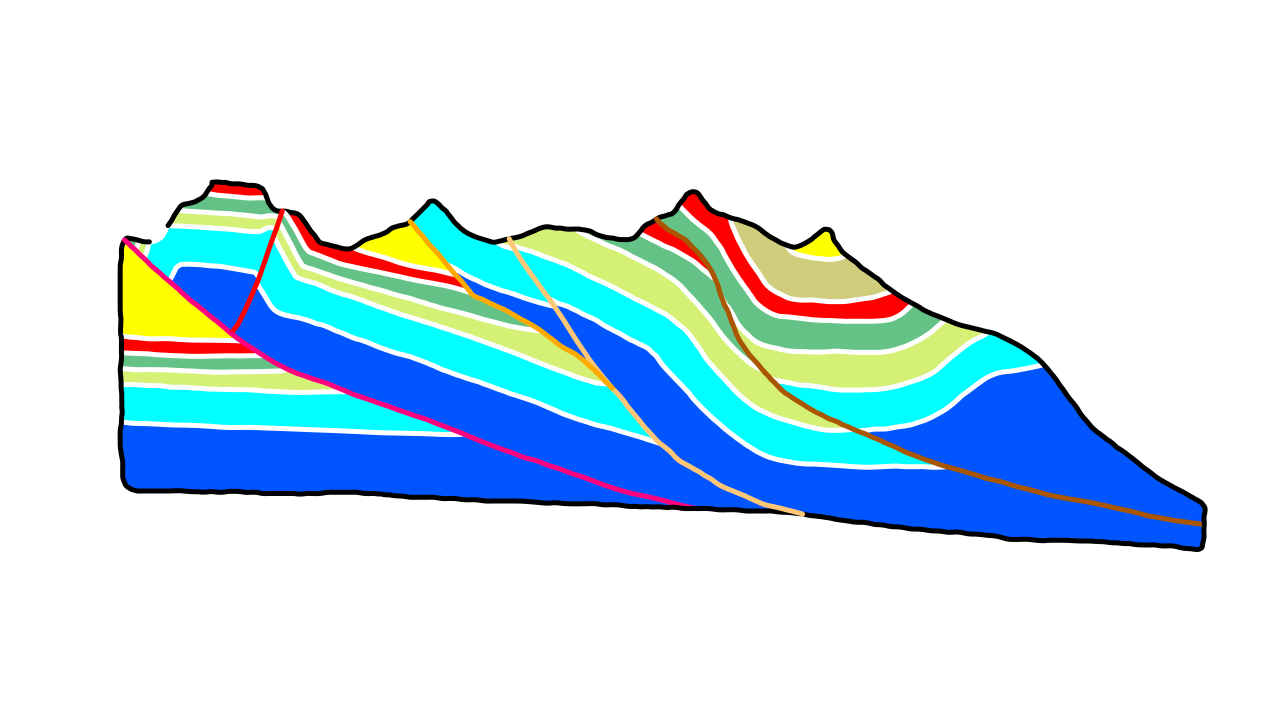
\includegraphics[scale=0.5]{chartreusevpaint.png}
	\caption{Chartreuse section drawn with VPaint}
\end{figure}

We will use the precendently described geological structure as our intern cross section data structure. In other words a drawing will be represented as a cross section which will be composed of blocks themselves composed of units. Because we consider that at the restoration state all units are straight rectangles, we decompose our units into two sides (left and right) and two level boundaries (upper and bottom) which either make the links between unit or constitute the limits of the drawing. 
%drawing

 \begin{figure}[H]
	\centering
	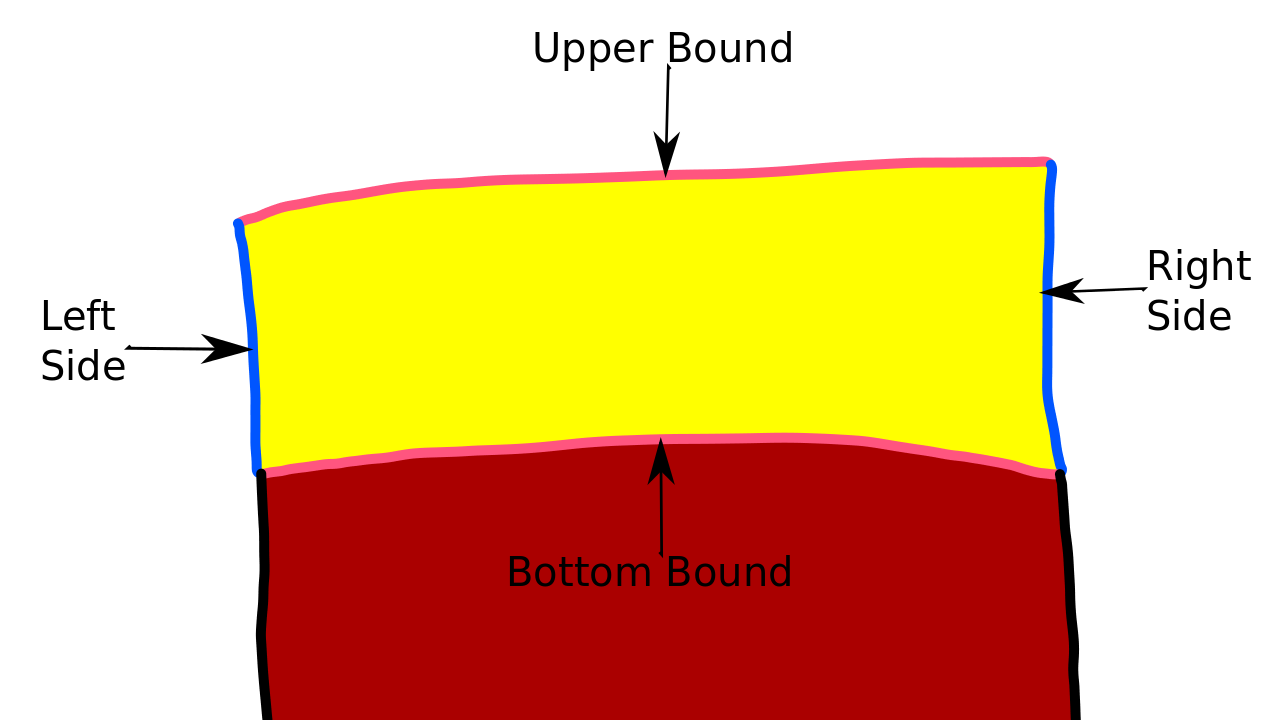
\includegraphics[scale=0.3]{unitDescriptionEdit.png}
	\caption{Geological unit representation}
\end{figure}

Thus we must deduce those structure from the input vpaint file. \\\\\
To do so we use the colors of our edges and faces. When importing the drawing we first ask to the user to give the different time period for each material exisiting in the cross section. Then we will build our blocks by adding succefully all the unit of each layer starting the youngest ones to the oldest. We do this sort in order to simplify the block creation and minimize the number of block created during this phase. Moreover when adding a new unit we try to find one already added unit which share either one portion of its upper bound  or its bottom bound with it. If we can't find one matching unit we place it in a new block. If we find one or several sharing units we deduce that they are all part of the same block so we store them in one unique block. If we do the sort like previously enonced we will thus reduce the number of block created because the only cases where we create blocks are either when the newly added unit is a surface unit or is unit located in a different block than the previously added ones.\\\\

When we have all our blocks created in our internal stucture we can identify the fault by looking at the color of the edges. If it is different than black or wite then it correspond to a fault which are caractarised by they color. The units are caracterized by their face color and their upper and bottom bounds which are drawn in white for most of them. Cross section border are usually drawn in black but we can deduce automatically which edge belongs to the lacking bound (limitation it is not always good).\\\\

We then have all the different material age, the blocks and units objects and the different fault we can find in the drawing. We will store all these information into a configuaration file .geo which will allow the user to save time by not giving the material information each times he opens the file. We have to note that in the input XML file, faces have an arbitrary cycling orientation which can be clockwise or counterclockwise. That's why but for building and manipulating our structure more easelly we will choose the convention that all our units will be first read clockwiselly. Thus we reverse the faces which are written counterclockwisely\\\\

\section{General Overview}

Here we will present our first method to tackle the problem of proposing a panel of plausible animations giving geological restoration as final state from a 2D input slice. 
The main idea of our methods is to map a mass spring system on each block of the cross section applying an implicit euler scheme solving the Newton's second law while possibly freezing the physic of several blocks at each time step regarding the undoing geological event. The output of our method we will a series of inbetween VGC encoded in a VAC which will be played on VPaint.\\\\
After drawing our section in VPaint we will read the XML output file in our tool  and add all the necessary information needed by the simulation as the layers' materials one containing in particular their deformation and friction coefficients. This information will allow us to run the animation over our section.\\

\section{Animation Model}

Like mentionned above the animation will be done by mapping a mass-spring system on each block. In fact it is more accurate to say that mass-spring system are mapped on layers instead of blocks. We proceed this way to take into account each layer orientation in the mapping as it is mapped according to layer's borders gradients. Considering that each layer is a rectangle that underwent some deformations the mapping will be done following the steps:	\\\\		
\indent	- First we have to put the masses both at the layer border but also inside it.\\\\
\indent	- We put the masses on the borders in an uniform way.\\\\
\indent	- We put the masses inside the layer: to do so we have two solutions:\\\\
\indent \indent	- Compute Hermite curve between each pair mass of the two level bounds and place particles uniformly on those curves.\\\\
\indent \indent	- Compute the intersections between the previous Hermite curves and the one coming from each pair mass of the two sides and place particles at those intersections.\\\\
	Even if the second solution might show better results that the first one we have chance that the curve comming from the sides might be not inside the layer due to big deformation making the layer non convex. \\With the first solution this problem is unlikely to occur because of the type of the deformations. In either case the Hermite curves be created using a mass pair and the gradient of the broder at each extremity as tangents. This way the layer will tend to transform back to a rectangle shape.\\\\
\indent	- Link particles with springs. \\\\We divide springs into 5 categories like described in \citep{cloth}: Vertical, Horizontal, DownShear, UpShear and Flexion. Adding flexion spring show better results in terms of shape preservation and breaking prevention. The resulting network looks like:\\
	
	\begin{figure}[H]
	\centering
	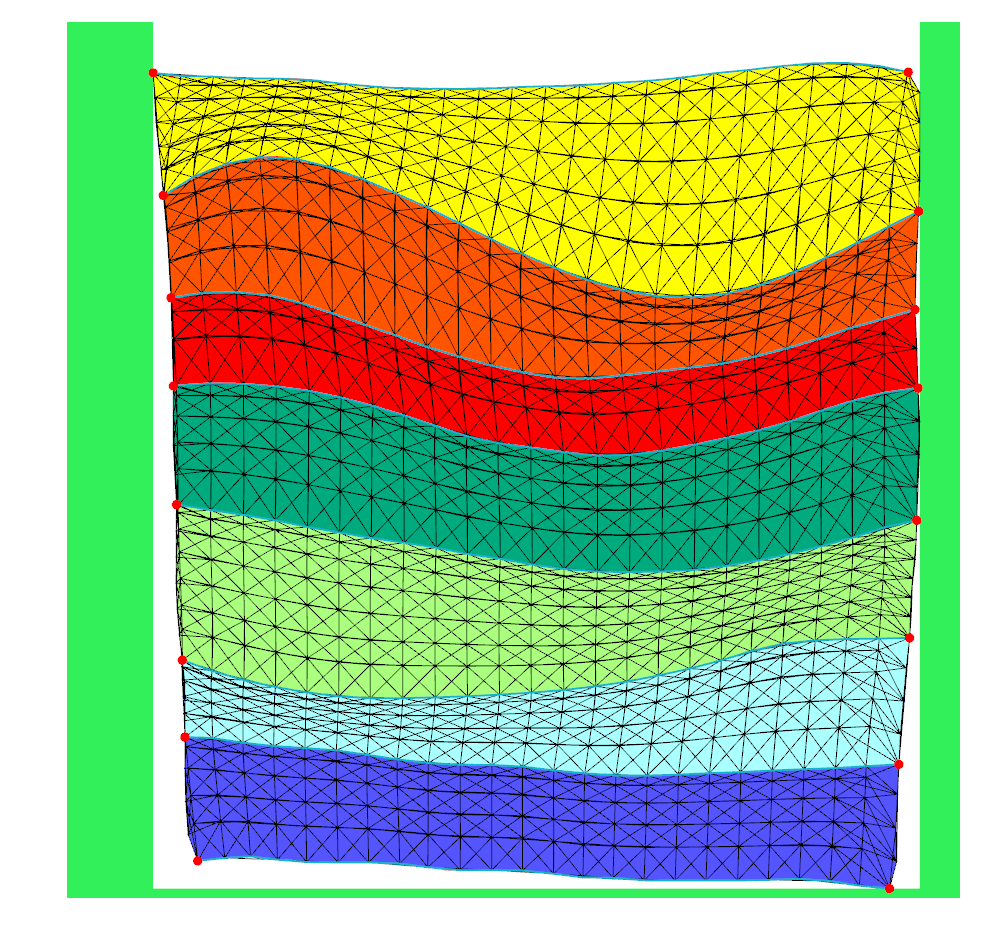
\includegraphics[scale=0.5]{springMapping.png}
	\caption{Mass-Spring Mapping on a layer. In purple: interlayers. In white: sides}
	\end{figure}
	
	\indent	- In addition the stiffness of the springs which affect the way the unit deforms will be proportionnal to the unit material Young modulus. \\\\
\indent	- The springs we use will also have a torsion resistance in order to accentuate the shape change of the layer.\\\\
In terms of physical equations for a single mass spring system we use the implicit euler scheme and algorithm descibed in \citep{caltech}. We use this scheme instead of an explicit one because it is proven to be more stable with big time step ($dt = 0.02$).\\\\ 
Each particle has the same mass $m$ and possesses at step $n$:\\\\
\indent	- A position  $x_i^n$\\\\
\indent	- A speed $v_i^n$ \\\\\
\indent	- Applied forces $F_i^n$ (containing filtered, corrected and external forces).\\\\
At each time step we will solve the second Newton's law:\\

\begin{align}
	v_i^{n+1} &= v_i^n + F_i^{n+1} \frac{dt}{m}\\
	x_i^{n+1} &= x_i^n + v_i^{n+1} dt 
\end{align}

with:

\begin{equation}
F_i^{n+1} = - \sum\limits_{j|(i,j)\in Edges} k_{ij}(x_i - x_j) + k_{ij}l_{ij}^0\frac{(x_i - x_j)}{||(x_i - x_j)||}
\end{equation}


For each particle we want to integrate the above equations. The problem is that we don't know the forces at step $n + 1$ as we don't know the position of the particles at this step. That is why we use a first order approximation to solve the problem at step $n + 1$:

\begin{equation}
	F^{n+1} = F^n + \frac{\partial F}{\partial x}(x^{n+1} - x^n)
\end{equation}

\noindent Thus we need to compute $H =  \frac{\partial F}{\partial x}$ which is the Jacobian of $F$.\\\\
\noindent By using (1) and (4) we have the following result:
\begin{align*}
	(x^{n+1} - x^n) &= (v^n + (v^{n+1} - v^n))dt \\
	(v^{n+1} - v^n) &= (I - \frac{dt^2}{m}H)^{-1}(F^n + dt H v^n)\frac{dt}{m}
\end{align*}

We now have approximated our equations into a solvable system and we can notice that an additionnal force came from this approximation $dt H v^n$ . It is an implicit viscosity that takes into account the movement of the neighbouring particles.
Consequently we have for each particle $i$ a new force:

\begin{equation}
\tilde{F_i} = k dt \sum\limits_{j|(i,j)\in Edges}(v_j - v_i)
\end{equation}


The last thing to compute is $H$. Like in \citep{caltech} we will approximate $H$ by just integrating the linear part of the elastic force which is equal to:

\begin{equation}
F_{(i,j)} = -k_{ij}(x_i - x_j) + k_{ij}l_{ij}^0\frac{(x_i - x_j)}{||(x_i - x_j)||}
\end{equation}

If $H$ represents only the Jacobian of $F = -k_{ij}(x_i - x_j)$ it has the form:\\
\begin{center}
$
\left\{
\begin{array}{ll}
H_{ij} &= k_{ij} if i \neq j \\
H_{ii} &= -\sum\limits_{j \neq i}k_{ij}
\end{array}
\right.
$
\end{center}

Integrating only the linear part implies that we will have some error at the end of the integration. However we can notice that the non linear part $k_{ij}l_{ij}^0\frac{(x_i - x_j)}{||(x_i - x_j)||}$ has a constant magnitude during the simulation between two steps, so this force just implies a rotation that we will compensiate with another force. Thus we will correct the angular momentum $\delta T$ introduced by this method by adding correcting forces:
\begin{align*}
\delta T &= \sum\limits_{i=1}^n (x_G - x_i)\wedge F_i^{filtered} \\
F_i^{corrected} &= (x_G - x_i)\wedge \delta T dt
\end{align*}

with:
\begin{equation}
F_i^{filtered} = \sum\limits_{i=1}^n F_{ji}W_{ij}
\end{equation}

However in our case the equilibrum length of the springs will change over time creating an error in the angular momentum but we will try compensating this with torsion forces.\\\\

Finally we add torsion forces as external forces (along with gravity) because it is a non linear force and we can't integrate it:

\begin{equation}
F_{ij}^{torsion} = -k_{torsion}\Delta \theta \vec{n}
\end{equation}

with $\Delta \theta$ being the angle between a unit vector depending on the spring type (Vertical, Horizontal, DownShear or UpShear) and the vector $x_i - x_j$. $\vec{n}$ is the normal vector to $x_i - x_j$ pointing toward the unit vector.\\\\

Finally we can add a optionnal inverse dynamic step at the end of the scheme loop which consist in correcting spring angles which make quads or triangles to be inverted causing face self intersection. Actually the torsion we already apply helps to prevent for having this case it is not given. Consequently here we impose that $\theta < \frac{\pi}{2}$ 

Computing a mass spring system can take some time (few seconds for big systems) and can be noticable especially during block fusion but that is not a problem because the goal of the project is to record at each time step the result of our simulation as an inbetween VAC which can be played fluently.\\\\

\section{Dealing With Discrete Geological Events}\\

As we mentionned earlier, geologists are usually able to restore the history of cross sections by using several geometrical and simulation tools. However they only get one sequence leading to the final state of the section which represents its the state before any techtonic movement. Here we are interested in what happened between today's section state and the restoration. Indeed most of the time, when restoring sections; there are several scenarios that lead the initial state to the restoration, that is why geolists often question others' hypothesis. This is exactly one of the main thread of this project. We want to explore the most plausibles scenarios and see the resulting animation of exploration.\\\\
To do so we will propose to the user to undo geological events at each time step. We can count already four events we want to undo : faults, erosion, sedimentation and  folding. Those events will be automatically detected and resorbed most of the time. It is possible to detect automatically faults, erosion and sedimentation but folding is something not present in the drawing, the applied forces are not shown. Therefore the user has to provide the un-folding even, meaning he has to choose when and how we want to apply it.\\\\ 

In order to encode our events in a intuitive manner we will use a story tree. However given the cross section we must determine the possible events to undo but also their time dependency with each other. For instance we know that the last event we will undo will be a sedimentation , that is why this un-sediment event must come after un-erode or un-fold events if this kind of event occured. In order to take into account this time dependency between events we will use an Event Graph to encode it. On the other hand, the story tree will be stored within a Story Graph which will be build thanks to the Event Graph and progressively expanded by the user.\\\\

The Story graph represents the different event sequences we can run the simulation on. A node represents the list of event we can simulate at time $t$ and an edge represents the events simulated between two nodes. The Event Graph is used in the creation of this Story Graph be cause it will be taken into account when proposing at time $t$ the list of possible event to simulate. As a result user will explore this graph as a tree and will be able to see the animation of as many scenarios as he wants to see.\\\\

Here is an example of Story Graph generated on a simple example:
%example story graph


Having a structure to create and come back on scenarios, we have to simulate the chosen events. To do so we have to set up the event structure which will allow the event to begin, being simulated and to end.\\\\

In order to simulate an event, it has to fulfill preconditions which are required for the simulation and to ensure geological consistancy. Then when an event is simulated it has also post conditions to fulfill in order to transform the cross section into the state it was before this event. With this convention, simulating an event is equivalent into inbetweening the section from the precondition to the postcondition state. Furthermore all the simulated events evolve in the same time line having a duration which can be set by the user depending on the event.\\\\

During this thesis we identified 4 events we could simulate with our given input data: un-erode, un-sediment, un-fault and un-fold. Each event has a very specific way to be simulated using the mass-spring model we introduced as its base.\\\\

Here we presents the way of simulating those events:

\subsection{Un-Sediment}

Un-sedimenting a layer consist in removing sediment progressively when the upper bound of the layer is perfectly horizontal as it is an unbreakable rule in geology.\\\\

In a sequence we will simulate the layer's thickness shrinking like:
%Dessin
\textbf{Precondition:} the layer's upper bound must be horizontal and the layer must be the youngest in the section.\\\\
\textbf{Simulation:} we progressively decrease the equilibrium length of vertical springs until it reaches $0$ for all the vertical springs when the event end.\\\\
\textbf{Duration:} given by material's age we want to un-sediment.\\\\
\textbf{Postcondition:} the layer must have desappeared letting a new layer to be the youngest 
in the section.\\\\
\textbf{Postcomputation:} regenerate the mass-spring system of the containing block at the end of the event.\\\\

\subsection{Un-Erode}

In the cross section the erosion impact can be noticed by variation of thickness in the same layer. However, it can have different effects topologicaly speaking depending on where it is applied. Here we will distinguish three different categories of erosion because of their topological and geometrical effects.\\\\

\subsection{Un-Erode block side}

Here we are interested in the erosion that occured at the side of the blocks which creates concavites and reduce the thickness of layers at some places. Here we will try to fill the concavities we can detect if they appear to have been created by an erosion process such as:

%dessin
This event is applicable to any surface module of the cross section.\\\\
\textbf{Precondition:} A concavity must be detected in the unit's sides. Here we are not interested in detecting all the concavities in the sides because some of them might have been caused by other events than erosion such as folding. Moreover we are interested in concavities which are between the upper corners of the units and its side. To be more precise we will fill an area between a upper side corner and the farthest side particle where there is a concavity in between. Progressively starting by the upper masses of the side and going down, we will look at the segment between the upper corner of the side and the considered particle. If the segment do not intersect the unit itself, then it is considered as a concavity. The final segment which we are interested in is the concavity segement between the corner and the farthest particle on the side. We store this particle and if it is different from the particle right after the corner then it means that there is a concavity to fill and the precondition is fulfilled.\\\\
\textbf{Simulation:}  Starting from this found farthest particle, we will compute the normal att his point and create a new mass following the line beginning at the found particle and directed by the normal. The new mass will be created at the point of same high than the upper corner in the normal line. This point will be the new corner of the unit and expand it as the new side will be projected toward the computed normal line.\\\\
\textbf{Duration:} given by the user.\\\\
\textbf{Postcondition:} the side that has been un-eroded must not intersect other units.\\\\
\textbf{Postcomputation:} regenerate the mass-spring system of the containing block at the end of the event.\\\\

\subsection{Un-Erode surface upper bounds}

Having treated the case of side erosion, we want also to un-do erosion that affected the upper surface of layers. Here concavities are not the only target we want to focus on. In this case erosion can easely let the surface being convex, so we will try to detect zones where the thickness of the layer decreased. Therefore we will look for zones in the upper bound where the curvature suddenly changed.\\\\
%dessin
\textbf{Precondition:} the upper bound must be at the surface and must have either a concavity or a changing curvature at some point. To detect convaties this time we use mathematical properties of the upper bound curve because we don't want to miss one as any concavity can be a product of erosion in this case. Therefore we look at the upper bound as being a discretized parametric curve $(x(t),y(t))$ and we search for concavities. To do so we will compute the speed vector $(x'(t),y'(t))$ and the acceleration vector $(x''(t),y''(t))$ and look at the sign of $det(v(t),a(t))$. If it is negative it means that the curve is concave. Thus we search for every concave areas which are intervals $[t_0,t_1]$ where the the curve is concave. We can also check if the curve has a big change in its curvature and if this change doesn't create a concavity. This is likely to happen  in holes which dug through several layers. Here the eroded part of the surface upper bound is likely to be eroded even being convex. Here the change in curvature might be noticable and we propose to the user to un-erode those units when we detect such a unit configuration. As a consequence whenever we detec a surface bound in a hole which divided at least one unit into two we propose the un-erode event for a part the surface curve in an interval $[t_0,t_1]$ just like before.\\\\
\textbf{Simulation:} In both cases we will use Hermite curve to fill the lacking matter. We will use them with the following coefficients $I(t_0), I(t_1)$ which are the points at the beginning and the end of the eroded curve and $I(t_0) - I(t_0 - 1), I(t_1) - I(t_1 + 1)$  as tangent respectively at point $I(t_0)$ and point $I(t_1)$. Then we deform the current curve making it matching the computed Hermite curve. By proceeding this way we will fill abnormalities in the layers following the trajectory the curve should have if we un-erode it.\\\\
\textbf{Postcondition:} the abnormalities must have been filled.\\\\
\textbf{Postcomputation:} regenerate the mass-spring system of the containing block at the end of the event.\\\\
\subsection{Un-Erode two facing units of the same Material}

Here we are interested in the case where erosion happened in the middle of a layer, making a hole a dividing it into several units. We can note that this can happen for units which are in the same block but also for units in neighbouring blocks. Here we will merge the two divided unit by adding an interpolated part bewteen them.\\\\
%drawing
\textbf{Precondition:} the two units must face each other in all cases and not in contact in a fault if there are on different blocks. It is obvious that they should be of the same material. Finally if there are in a hole that divided older layers we cannot un-do this erosion before un-doing the erosion of those layers.\\\\
\textbf{Simulation:} Here we will use Hermite curve again for the same reason of preserving the curvature continuity. If we are in the case of units between blocks, we will use an Hermite curve joining the two upper bounds and one joining the two bottom bounds and fill the zone delimited by these two curves. If we are in the case of two units in the same block we only need to interporlate the upper bound as the bottom bound already exist.\\\\
\textbf{Postcondition:} the two units must have merged into a new one.\\\\
\textbf{Postcomputation:} regenerate the mass-spring system of the containing block at the end of the event.\\\\
\subsection{Un-Erode special case}

Finally we identified a last case of erosion which correspond to the following configuration.\\\\
%dessin
Here we can wonder if the yellow unit has been eroded.  It seems that there is lacking matter on the red unit and we want to add yellow sediment fill the surface part of this unit. However geologically speaking here we observe that the units are highly deformed and so the lacking part might not be one and the yellow sediment has only deposited in the left side because of relief shape. In the case we want to un-erode  the yellow unit we have add enough matter to fill all the red unit surface.\\\\
\textbf{Precondition:} the concerned unit must have free surface upper bound of the unit just under him.\\\\
\textbf{Simulation:} Here we just extend the concerned unit until the end of the free surface while increasing its thickness if it is necessary for filling the lacking part.\\\\
\textbf{PostCondition:} All the free surface bound must have been filled by the concerned unit sediment.\\\\
\textbf{Postcomputation:} regenerate the mass-spring system of the containing block at the end of the event.\\\\
\subsection{Un-Fold}

Un-Folding basically means applying forces on blocks, units or particles of the section. Theses forces can be applied in any manner such as uniformly or linearly. It is a event which is most of the time added by the user but plays also a major role in the un-fault event.\\\\
%dessin
\textbf{Precondition:} there are no preconditions for this event. the user is free to play with this event as it allows geologists to test their hypothesis on forces that have been applied to the section in the past.\\\\
\textbf{Simulation:} We add external forces either to a block, a unit or a specific mass during the requested time. The external forces are taken into account in the main physical loop.\\\\
\textbf{Duration:} given by the user.\\\\
\textbf{Postcondition:} he event no longer apply forces on the concerned particles.\\\\

\subsection{Un-Fault}

Here we will describe the un-fault event which has special feature of been a composed event. Indeed we considered that the un-fault event is the concatenation of three events: un-erode, un-slide and un-fold. As an un-fault event can only occur between two blocks (and only two) we will proceed by first un-eroding units which are not in contact and then making one block sliding on the other while un-folding the whole cross-section. We can note that when an fault occur, it breaks one block starting by the oldest layer to the youngest. We will use this property to decompose our un fault event into several stickUnits events for units we don't un-erode at the beginning of the un-fault event.\\\\
% dessin
Before explaining the un-fault event, we will present the simple stickUnit event. There are no preconditions has it is the created and called by the fault event which manage preconditions. This event wait for matching unit to be face to face and merge them when there are. In addition as fault can be created by extreme folding condition we apply an little attraction force on the sliding unit in order to fold it like it was at the moment of the break. Thus we apply $\overrrightarrow{F} = d*\frac{\overrightarrow{(C_{lower} - C_{upper})} }{||\overrightarrow{(C_{lower} - C_{upper})}||}$ to the corners of the sliding unit going toward the corresponding corners of the matching unit.\\\\
We can now detail the un-fault event.\\\\
\textbf{Precondition:} The fault must be between two blocks and only two of them.\\\\
\textbf{Simulation:} We first ask the user if he wants to un-erode units which are not in contact in the fault using the "Un-Erode two facing units of the same Material" algorithm we describe before. Then we create the stickUnits event for each matching unit, they will be simulated one after the other starting by the youngest units to the oldest. At the same time we will let one block to slide on the other (the upper one in the case of the compression, the lower one if it is an extension) and fold on one extremity of the cross section depending if we are in a compression or extension and depending the direction of folding. This event ends when all the stick events have also ended.\\\\
\textbf{Postcondition:} all the sticking events ended meaning that all matching units merged together one new unit. That implies that the two concerned blocks merged.\\\\
\textbf{Postcomputation:} regenerate the mass-spring system of the containing block at the end of the event for a better mesh uniformity.\\\\ 
		
\section{Scheduling and Proposing Events}

We presented how the different events are simulated and how the user can choose different scenarios. We will now present the way of proposing the possible events using the Event Graph and some other techniques in order to give the user the means for restoring the cross section.\\\\

When loading the vpaint cross section we are able to identify events to undo  and create time dependencies between them just by looking at the geological and geometrical properties of the section. For instance we can sort the un-sediment events by looking at the material ages, the youngest sediment will be the first one the user will un-sediment and the oldest will be the last. We can go further and look at erosion and faults. It is obvious that un-erode events of one material must occur before its un-sedimentation. As for faults, we can look at them and see if there are units of blocks which are already stick together. Indeed a fault always shifts a matching unit (of the same material) by a offset when it is playing. However if the fault stop playing and if the sedimentation continue we will have already stuck units from both sides of the fault just like this example:\\\\
%example

Thus we can conclude that the fault occured before the new sedimentation and record it in the Event Graph.\\\\

Here is an example of an event graph for a simple example:\\\\

However, while it is possible to identify events beforehand, some others are only detectable at a given moment $t$. For instance un-eroding concave part is only detectable at a given moment because concavities can appear and disappear while the whole terrain is deforming by un-doing other events. As a consequence at each time step where an un-do event ends we have to detect this kind of event and propose it to the user. We will call this kind of event Dynamic event as they only exist at a given proposition. In addition events such as un-Fold are not always detectable and must be given to the hand of the user. That is why will we give him the opportunity to add its own Dynamic events when choosing among the list of possible events. Those events will be denominated as User Events.\\\\

Now that we presented how to schedule the events we will propose a method to build the list  at each proposing step. The first proposal will contain the events of the Event Graph which do not have any other event depending on them and respect their un-doing precondition, meaning that they are likely to be the last events that occured in the time direct way, thus to be the first events to un-do. Then we add the detected dynamic events and the user ones and we obtain our first proposal. Starting this first list the user makes its event choice and we wait until the choosen events end. We then have to generate a new list of possible event. To do so we will add the events which our previously choosed event depended on and which respect their precondition, meaning that we will propose events which occured before (in the time direct way) the event we just un-did. Then we add our Dynamic and User event and we completed our list. Then we just proceed this way until the list of possible event is empty or until the user wishes it.\\\\\

However by proceeding this way the list of possible will be very big at each proposal in average. That's why we have to cut branches of the Story Tree by erasing events which have a little probability to occur and encourage the user to explore the branch which have the biggest probability to occur; thus we propose a branch and bound method to the user to explore the different scenarios of our cross section restoration.\\\\

As a consequence we must build evaluation function for each proposed event which will return its probabilty to occur. Here is some example of what can be an evaluation function for our geological case:\\\\

 - Un-fault: We compute the side length of each of the two blocks' units which are in contact at the fault. The little the sum of the differences of each same material unit side length is the greater is the probability for the un-fault event to occur. It is justified by the fact that when a fault is closing it is done almost instantly with all the matching units facing each other\\\\
 
 - Un-eroding a concavity: the wider the concavity is the greater the probability of occurrence is for this event. It is justified by the fact that keeping units having the same thickness on all their length is important to go back in time because at the restoration time they have the same thickness every where for the same material. Thus big eroded part must be the first ones to un-erode in order to assure the success of the simulation.\\\\
 

\section{Implementation}

\section{Results}
\section{Limitations}
- 3D with more Cross sections\\
- Could have used clothoid for preserving layer thickness\\
- Sequential and not list of un-doing events\\
- Let the user draw erosion line -- already determined eroded zones\\
- Thickness limitation: it is not geologicaly good because we don't look at the layer thickness.
\section{Conclusion}



\section{Annex}

Hermite curves equations :\\
Given two points $P_0, P_1$ and two tangents $T_0, T_1$ being the tangent we can find at the matching number points, the Hermite interpolation which will produce a $C_1$ curve has for equation : 


\begin{equation}
h(t) = (2*t^3 - 3*t^2 + 1)*P_0 + (t^3 - 2*t^2 + t)*T_0 + (t^3 -t^2)*T_1 +(3*t^2 - 2*t^3)*P_0
\end{equation}

It is possible to multiply the tangent by a bias factor which will make the curvature of the curve varying more when this factor becomes big.

Collisions methods: \\

Collisions between blocks. Each layer is delimited by its boundaries which we devide into four parts: upper interlayer, bottom interlayer, right side and left side. Each of these part are composed of segments and the union of all of them is a closed polygon. We deal with block collision by computing particle (circle) segments collision. Moreover for each particle of one block we consider the segement built by the particle position at time $t - dt$ and its position at time $t$ and we check if this segment crosses one of the other blocks segment border. In addition, with this we can also check for collision inside the block it self which is usefull to give reallistic results for un sedimentation for instance. This technique as the advantage of determinig precisely the segment with which the particle collided even if the particle went through the colliding block. However there is still a chance to fail at identifying a collision depending on the order we treat each block animation and collision detection.\\
In order to check intersection between segments we proceed the following way:\\
Given two sgements $[PQ]$ and $[RS]$ we will consider a parametrisation of their equations: 

\begin{align}
	PQ &= P + t*\overrightarrow{PQ} \forall t \in [0,1]\\
	RS &= R + u*\overrightarrow{RS} \forall u \in [0,1]\\
\end{align}

With this parametrisation the two segments intersect if and only if:\\
\begin{equation}
\exists t,u \in [0,1], P + t*\overrightarrow{PQ} = R + u*\overrightarrow{RS}
\end{equation}


We need to extract two equations from this one in order to find $u$ and $t$.
To do so we will use the cross product to keep only one variable in each equation. Thus by applying a cross product with $\overrightarrow{PQ}$ and $\overrightarrow{RS}$ we obtain the following equations:

\begin{align}
	t &= \frac{\overrightarrow{(R - P)} \wedge \overrightarrow{RS}}{\overrightarrow{PQ} \wedge \overrightarrow{RS}}\\
	u &= \frac{\overrightarrow{(P - R)} \wedge \overrightarrow{PQ}}{\overrightarrow{RS} \wedge \overrightarrow{PQ}}
\end{align}

We must note that the simplification was made by noticing that $\overrightarrow{PQ} \wedge \overrightarrow{PQ} = 0$ and $\overrightarrow{RS} \wedge \overrightarrow{RS} = 0$.

Then we can distinguish $4$ cases :\\\\
1) $ \overrightarrow{RS} \wedge \overrightarrow{PQ} = 0$ and $\overrightarrow{(P - R)} \wedge \overrightarrow{PQ} = 0$\\\\
This means that our segments are parrallel because of the first condition and colinear because of the second. We deduce that our segement are intersecting if: \\\\ 
($\overrightarrow{PR}.\overrightarrow{PS} < 0$) or ($\overrightarrow{PR}.\overrightarrow{PS} \geq 0$ and $\overrightarrow{PQ}.\overrightarrow{PS} \geq 0$ and ($||\overrightarrow{PS}|| < ||\overrightarrow{PQ}||$ or $||\overrightarrow{PR}|| < ||\overrightarrow{PQ}||$))
\\\\\
2)  $ \overrightarrow{RS} \wedge \overrightarrow{PQ} = 0$ and $\overrightarrow{(P - R)} \wedge \overrightarrow{PQ} \neq 0$
In that case the segeents are parallel but non intersecting.\\\\
3)  $ \overrightarrow{RS} \wedge \overrightarrow{PQ} \neq 0$.
The segment are intersecting iff the computation of $t$ and $u$ gives $t,u \in [0,1]$\\\\
4) Otherwise the segements are not parallel and non intersecting\\\\
\begin{figure}[H]
	\centering
	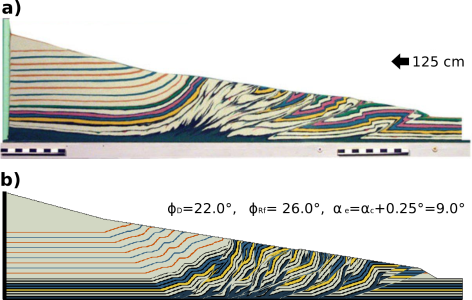
\includegraphics[scale=0.5]{slamtec.png}
	\caption{Slamtec cross section modeling}
\end{figure}



\bibliography{pfe.bib}

\end{document} 